% presentation
\documentclass{beamer}

\usetheme{Warsaw}

% rus lang
\usepackage[main=russian,english]{babel}

% insert images
\usepackage{wrapfig}

% declare operator
\DeclareMathOperator*{\argmin}{argmin} % thin space, limits underneath in displays
\newcommand{\at}[2][]{#1|_{#2}}

% alrorithm
\usepackage{algorithm2e}
\usepackage{algorithm}
\usepackage{algpseudocode}
% \usepackage{algorithmic}

% math
\usepackage{amsmath}
\DeclareMathOperator{\sign}{sign}
\DeclareMathOperator{\K}{K}

\title[Классификация]{Лекция 3. Классификация}
\subtitle{Основы интеллектуального анализа данных}
\author{Полузёров Т. Д.}
\institute{БГУ ФПМИ}
\date{}

\begin{document}
	
	\begin{frame}
		\titlepage
	\end{frame}
	
	\begin{center}
		\frametitle{Структура лекции}
		\tableofcontents	
	\end{center}
	
	\section{Байесовские методы}
	
	\begin{frame}
		\frametitle{Вероятностная постановка задачи}
		 $\mathbb{X}$ - множество объектов, $\mathbb{Y}$ - множество классов.
		 
		$(\mathbb{X} \times \mathbb{Y})$ - вероятностное пространство с совместной плотностью $p(x, y) = P(y) p(x | y)$
		 
		$P_y := P(y)$ - \textbf{априорные вероятности} классов (prior)
		
		$p_y(x) := p(x | y)$ - \textbf{функции правдоподобия} классов (likelihood)
		
		\vspace{15pt}
		
		Задачи:
		
		\begin{enumerate}
			\item По выборке $(X, Y) \in (\mathbb{X}, \mathbb{Y})$ построить оценки распределений $\hat{P_y}$ и $\hat{p_y}(x)$
			\item По известным распределениям $p_y(x)$ и $P_y$ построить алгоритм $a: \mathbb{X} \rightarrow \mathbb{Y}$ минимизирующий вероятность ошибочной классификации
		\end{enumerate}
	\end{frame}
	
	\subsection{Оптимальный классификатор}
	
	\begin{frame}
		\frametitle{Функционал среднего риска}
		Алгоритм $a(x)$ разбивает $\mathbb{X}$ на непересекающиеся области $A_y = \{x \in \mathbb{X} | a(x) = y \}$
		
		\vspace{10pt}
		
		Каждой паре $(y, s) \in (\mathbb{Y} \times \mathbb{Y})$ соответствует величина потери $\lambda_{ys}$ при классификации объекта класса $y$ к классу $s$, $\lambda_{yy} = 0$ и $\lambda_{ys} > 0$ при $y \ne s$
		
		\vspace{10pt}
		
		\textbf{Функционал среднего риска}:
		
		 \[
		 R(a) = \sum_{y \in \mathbb{Y}} \sum_{s \in \mathbb{Y}}
		 \lambda_{ys} P_y P(A_s | y)
		 \]
		 
		 где $P(A_s | y) = \int_{A_s} p_y(x) dx$ - вероятность отнесения к классу $s$ объекта класса $y$.	 
	\end{frame}
	
	\begin{frame}
		\frametitle{Теорема о минимуме среднего риска}
		% теорема
		
		Если известны априорные вероятности $P_y$ и функции правдоподобия $p_y(x)$, то минимум среднего риска
		\[
		R(a) = \sum_{y \in \mathbb{Y}} \sum_{s \in \mathbb{Y}}
		\lambda_{ys} P_y P(A_s | y)
		\]
		
		достигается алгоритмом
		
		\[
		a(x) = \arg \min_{s \in \mathbb{Y}} \sum_{y \in \mathbb{Y}} \lambda_{ys} P_y p_y(x)
		\]
	\end{frame}
	
	\begin{frame}
		\frametitle{Байесовское решающее правило}
		Если предположить что потери от ошибочной классификации зависят только от истинного класса объекта, т.е. $\lambda_{ys} = \lambda_{y}$, то алгоритм называется \textbf{Байесовским решающим правило}:
		
		\[
		a(x) = \arg \max_{y \in \mathbb{Y}} \lambda_{y} P_y p_y(x)
		\]
	\end{frame}
	
	\begin{frame}
		\frametitle{Апостериорные вероятности}
		Вероятность $P(y | x)$ - называется \textbf{апостериорной вероятностью} (posterior).
		
		\vspace{10pt}
		
		Зная $p_y(x)$ и $P_y$, то по формуле Байеса:
		
		\[
		P(y | x) = 
		\frac{p(x, y)}{p(x)} =
		\frac{p_y(x) P_y}{\sum_{s \in \mathbb{Y}} p_s(x) P_s}
		\]
		
		\vspace{15pt}
		
		Величина ожидаемых потерь на объекте $x$:
		
		\[
		R(x) =
		\sum_{y \in \mathbb{Y}} \lambda_{y} P(y | x)
		\]
	\end{frame}
	
	\begin{frame}
		\frametitle{Принцип максимума апостериорной вероятности}
		Оптимальный байесовский классификатор через апостериорные вероятности:
		
		\[
		a(x) = \arg \max_{y \in \mathbb{Y}} \lambda_{y} P(y | x)
		\]
		
		\vspace{15pt}
		
		\begin{itemize}
		\item
		Если классы равнозначны ($\lambda_{y} = \lambda_{s} \forall y, s \in \mathbb{Y}$), то байесовское решающее правило называют \textbf{принципом максимума апостериорной вероятности}.
		
		\item
		В случае равновероятных (сбалансированных) классов ($P_y = \frac{1}{|\mathbb{Y}|}$), объект $x$ просто относится к классу с наибольшим значением плотности $p_y(x)$.
		\end{itemize}
	\end{frame}
	
	\begin{frame}
		\frametitle{}
		Получен оптимальный байесовский классификатор
		\[
		a(x) = \arg \max_{y \in \mathbb{Y}} \lambda_{y} P(y | x)
		\]
		Но плотности $P(y | x)$ неизвестны. Чтобы построить итоговый классификатор, ставится задача их оценить.
		
		\vspace{5pt}
		Основные подходы:
		\begin{enumerate}
			\item непараметрическое
			\item параметрическое оценивание плотности
			\item наивный подход
		\end{enumerate}
 		
	\end{frame}
	
	\subsection{Наивный подход}
	
	\begin{frame}
		\frametitle{Наивный подход}
		Суть наивного подхода - предположение о независимости признаков между собой.
		Это позволяет упростить
		
		\[
		P(x | y) = \prod_{i=1}^{n} P(x_i | y)
		\]
		
		Для построения итоговой плотности $P(x | y)$ нужно оценить все индивидуальные распределения признаков $P(x_i), i=1, ..., n$.
	\end{frame}
	
	\begin{frame}
		\frametitle{Наивный байесовский классификатор}
		Оценив априорные плотности и индивидуальные функции правдоподобия, получим \textbf{наивный байесовский классификатор}
		
		\[
		a(x) = \arg \max_{y \in \mathbb{Y}} \ln \lambda_{y} \hat{P}(y) + \sum_{i=1}^{n} \ln \hat{P}(x_i | y)
		\]
		
		Предположение о независимости признаков является очень сильным, но на практике почти никогда не выполняется. 
	\end{frame}
	
	\subsection{Непараметрическое восстановление плотности}
	
	\begin{frame}
		\frametitle{Одномерный непрерывный случай}
		Пусть $\mathbb{X} = \mathbb{R}$. 
		Эмпирической оценкой плотности есть доля элементов выборки внутри окна шириной $h$
		
		\[
		\hat{p}(x) = \frac{1}{2mh} \sum_{i=1}^{m} [|x - x_i| < h]
		\]
		
		Результат есть кусочно-постоянная функция. Это приводит к появлению зон неуверенности оптимальном классификаторе. Идея состоит в применении ядра
	\end{frame}
	
	\begin{frame}
		\frametitle{Ядерная оценка плотности}
		Функция $K(z)$ называется ядром, если она чётная и нормированная $\int K(z) dz = 1$
		
		\vspace{5pt}
		
		Тогда \textbf{ядерная оценка плотности} имеет вид:
		
		\[
		\hat{p}_h(x) = \frac{1}{mh} \sum_{i=1}^{m}K(\frac{x - x_i}{h})
		\]
		
		Примеры ядер:
		\begin{itemize}
			\item $K(z) = \frac{1}{2} [|z| < 1]$- прямоугольное
			\item $K(z) = \frac{1}{\sqrt{2\pi}} e^{-\frac{1}{2} z^2}$ -гауссово
		\end{itemize}
	\end{frame}
	
	\begin{frame}
		\frametitle{Многомерный случай}
		Ядерная оценка плотности для многомерной величины $X \in \mathbb{R}^n$
		
		\[
		\hat{p}_h(t) = \frac{1}{m} \sum_{i=1}^{m} \prod_{j=1}^{n} \frac{1}{h_j} \K (\frac{t - x_i}{h_j})
		\]
	\end{frame}
	
	\begin{frame}
		\frametitle{Метод парзеновского окна}
		Применяя ядерную оценку плотности в байесовском решающем правиле
		
		\[
		a(x) = \arg \max_{y \in \mathbb{Y}} \lambda_{y} \sum_{i=1}^{\ell} [y_i = y] K(\frac{\rho(x, x_i)}{h})
		\]
		
		где $\rho(z_1, z_2)$ некоторая функция расстояния между объектами
	\end{frame}
	
	\subsection{Параметрическое восстановление плотности}
	
	\begin{frame}
		\frametitle{Параметрический подход}
		Имеется выборка $X = (x_1, ..., x_{\ell}) \in \mathbb{X}$. Предполагается, что плотность, порождающая данные, известна \textbf{с точностью до параметра}, $p(x) = \phi(x; \theta)$. Подбор параметров $\theta$ приводится по выборке $X$ с помощью \textbf{метода максимального правдоподобия}.
		
		\vspace{15pt}
		
		\textbf{Нормальный дискриминантный анализ} - случай байесовской классифицакии в предположении о нормальном распределениии всех классов, $p_y(x) \sim N(\mu_y, \sigma_y^2), y \in \mathbb{Y}$.
	\end{frame}
	
	\begin{frame}
		\frametitle{Теорема о разделяющей поверхности}
		Если классы имеют $n$-мерные нормальные плотности распределения
		\[
		p_y(x) = N(x; \mu_y, \Sigma_y), y \in \mathbb{Y}
		\]
		то баейсовский классификатор задаёт квадратичную разделяющую поверхность.
		Она вырождается в линейную, если ковариационные матрица классов равны $\Sigma_y = \Sigma, y \in \mathbb{Y}$
	\end{frame}
	
	\begin{frame}
		\frametitle{Байесовский нормальный классификатор}
		Оценим параметры $\hat{\mu}_y$ и $\hat{\Sigma}_y$ $n$-мерной плотности  по имеющимся данным для каждого класса $y \in \mathbb{Y}$.
		
		\vspace{5pt}
		
		И воспользуемся идеей оптимального байесовского классификатора
		
		\[
		a(x) = \arg \max_{y \in \mathbb{Y}} \lambda_{y} P(y) P(x | y)
		\]
		
		\vspace{15pt}
		
		Такой классификатор называется \textbf{байесовский нормальный классификатор} или \textbf{подстановочный}
	\end{frame}
	
	\begin{frame}
		\frametitle{Линейный дискриминант Фишера}
		Предположив, что ковриационные матрицы классов равны $\Sigma_y = \Sigma, y \in \mathbb{Y}$ и применяя подстановочный алгоритм, получим метод линейного дискриминанта Фишера.
		
		\vspace{15pt}
		
		В таком случае разделяющая поверхность является линейной (в случае нескольких классов - кусочно линейная) и обладает определенными свойствами устойчивости.
	\end{frame}
	
	\section{Линейные методы}
	
	\subsection{Оценка сверху эмперического риска}
	
	\begin{frame}
		\frametitle{Бинарная классификация}
		Рассмотрим задачу бинарной классификации, $X=(x_1, ..., x_{\ell}) \in \mathbb{X}, Y \in \mathbb{Y} = \{-1, 1\}$
		
		\vspace{5pt}
		
		Функцию $a(x, \theta) = \sign f(x, \theta)$ будем называть \textbf{дискриминантной функцией}.
		
		\vspace{5pt}
		
		Если $f(x, \theta) > 0$, то $x$ относится к классу $+1$, 
		$f(x, \theta) < 0$ то $-1$. 
		
		\vspace{5pt}
		
		А множество точек $\{x | f(x, \theta) = 0\}$ - \textbf{разделяющая поверхность}.
		
		\vspace{5pt}
		
		Величина $M_i(\theta) = y_i f(x_i, \theta)$ - \textbf{отступ} (margin) классификатора $a(x, \theta) = \sign f(x, \theta)$ относительно объекта $x_i$.
		
		\vspace{5pt}
		
		Если $M_i(\theta) < 0$ то алгоритм $a$ допускает ошибку на объекте $x_i$. \textbf{Чем больше} $M_i(\theta)$ \textbf{тем правильнее} и надежнее классификация.  
	\end{frame} 
	
	\begin{frame}
		\frametitle{Функция потерь}
		Требуется подобрать параметры $\theta$ при которых классификатор $a$ допускает как можно меньше ошибок:
		
		\[
		Q(a, X) = \frac{1}{\ell} \sum_{i=1}^{\ell} [M_i(\theta) < 0] \rightarrow \min_{\theta}
		\]
		
		Однако в таком виде $Q$ - кусочно постоянная функция
		
		\vspace{15pt}
		
		Идея - мажорирование (оценка сверху) индикатора ошибки $[M_i(\theta) < 0]$ с помощью "удобной" функцией потерь $\mathcal{L}(M_i)$:
		
		\[
		Q(a, X) = \frac{1}{\ell} \sum_{i=1}^{\ell} [M_i(\theta) < 0]
		<=
		\widetilde{Q}(a, X) = \frac{1}{\ell} \sum_{i=1}^{\ell} \mathcal{L}(M_i(\theta))
		\]
	\end{frame}
	
	\begin{frame}
		\frametitle{Популярные функции потерь}
		\begin{enumerate}
			\item $[M < 0]$ - индикатор ошибки
			\item $(1 - M)^2$ - квадратичная
			\item $(1 - M)_{+}$ - кусочно линейная
			\item $\frac{2}{1 + e^M}$ - сигмоидная
			\item $\log_2(1 + e^{-M})$ - логистическая
			\item $e^{-M}$ - экспоненциальная
		\end{enumerate}
		%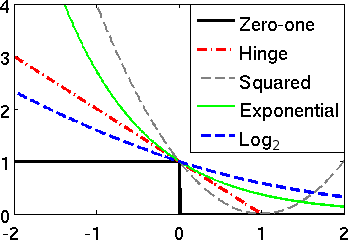
\includegraphics{img/loss_funcs.png}	
	\end{frame}
	
	\begin{frame}
		\frametitle{Функция потерь и совместное распределение}
		Пусть множество $(\mathbb{X} \times \mathbb{Y})$ - вероятностное пространосво. Имея выборку $(X, Y)$ и предполагаемый вид совместной плотности $p(x, y; \theta)$, применим метод максимального правдоподобия
		
		\[
		L(\theta) = \prod_{i=1}^{\ell} p(x_i, y_i; \theta) \rightarrow \max_{\theta}
		\]
		
		\[
		\ln L = \sum_{i=1}^{\ell} \ln p(x_i, y_i; \theta) \rightarrow \max_{\theta}
		\]
		
		\[
		- \ln p(x_i, y_i; \theta) = \mathcal{L}(y_i f(x_i, \theta))
		\]
		
		По виду плотности $p(x, y; \theta)$ восстанавливается $f$ и $\mathcal{L}$. И обратно, используя некоторые разделяющую поверхность и функцию потерь - предполагаем определенное распределение в данных.
	\end{frame}
	
	
	\begin{frame}
		\frametitle{Линейная модель}
		
		Случай $f(x, \omega) = \langle x, \omega \rangle$ - класс линейных моделей классификации.
		
		\[
		a(x, \omega) = \sign \langle x, \omega \rangle
		\]
		
		Разделяющая поверхность $\sign \langle x, \omega \rangle = 0$ является гиперплосткостью в $\mathbb{R}^{n}$. Причем объекты по одну сторону от гиперплосткости относятся к одному классу, по другую - к другому.
	\end{frame}
	
	\begin{frame}
		\frametitle{Метод обучения}
		Метод минимизации мажорированного эмперического риска 
		
		\[
		\widetilde{Q}(a, X) = \sum_{i=1}^{\ell} \mathcal{L}(\langle x_i, \omega \rangle y_i) \rightarrow \min_{\omega}
		\]
		
		Необходимое условие минимума:
		\[
		\frac{\partial Q}{\partial \omega} = \sum_{i=1}^{\ell}  x_i y_i \mathcal{L}^{'}(\langle x_i, \omega \rangle y_i) = 0
		\]
	\end{frame}
	
	\subsection{Логистическая регрессия}
	
	\begin{frame}
		\frametitle{Логистическая регрессия}
		Логистическая регрессия - линеный алгоритм бинарной классификации.
		
		При достаточно сильных свойствах обладает свойствами:
		\begin{itemize}
			\item оптимальный байесовский классификатор
			\item однозначно определена функция потерь
			\item возможность оценивать вероятности классов
		\end{itemize}
		
		Пусть $(\mathbb{X}\times \mathbb{Y}) = (\mathbb{R}^{n} \times \{-1, 1\})$ - вероятностное пространтсво с плотностью $p(x, y)$. Выборка $(X, Y)$ получена из этого распределения.
	\end{frame}
	
	\begin{frame}
		\frametitle{Экспонентный класс распределений}
		Плотность $p(x), x \in \mathbb{R}^{n}$ называется экспонентной, если
		\[
			p(x) = \exp(c(\delta) \langle \theta, x \rangle + b(\delta, \theta) + d(x, \delta))
		\]
		 где $\theta$ -параметр сдвига, $\delta$ - масштаба, $b, c, d$ - произвольные числовые функции.
		 
		 \vspace{15pt}
		 
		 Принадлежат к классу экспонентных:
		 \begin{itemize}
		 	\item Равномерное, Нормальное, Гамма
		 	\item Гипергеометрическое, Пуассоновское, Биномиальное
		 	\item и другие
		 \end{itemize}
	\end{frame}
	
	\begin{frame}
		\frametitle{Обоснование линейной модели}
		\[a(x) = \sign(\lambda_+ P(+1 | x) - \lambda_- P(-1 | x)) =
		\sign(\frac{P(+1 | x)}{P(-1 | x)} - \frac{\lambda_-}{\lambda_+})
		\]
		
		\textbf{Если} функции правдоподобия $p(x | y) $ принадлежат экспонентному классу, причем параметры $d$ и $\delta$ одинаковы, а отличаются только параметры сдвига $\theta$, 
		
		\textbf{то}:
		\begin{enumerate}
			\item байесовский классификатор является линейным: $a(x) = \sign \langle \omega, x \rangle$
			\item апостериорная вероятность $p(y | x) = \sigma(\langle \omega, x \rangle y)$
		\end{enumerate}
		
		где $\sigma(z) = \frac{1}{1 + e^{-z}}$ - сигмоидная функция, $\sigma(-z) = 1 - \sigma(z)$
	\end{frame}
	
	\begin{frame}
		\frametitle{Модель оценки вероятностей}
		Построим модель которая оценивает не сами метки классов, а \textbf{вероятности} принадлежности к ним.
		
		\[
		a(x, \omega) = P(+1 | x) = \sigma(\langle w, x \rangle)
		\]
		
		Другими словами, в каждой точке $x$ величина $y \sim Bernoulli(\sigma(\langle w, x \rangle))$
		
		\vspace{15pt}
		
		Задача классификации решается путем выбора порога $t \in [0, 1]$. И тогда итоговый классификатор имеет вид:
		
		\[
			b(x, t) = \sign (a(x, \omega) - t)
		\]
		
	\end{frame}
	
	\begin{frame}
		\frametitle{Метод максимального правдоподобия}
		С учетом вероятностной постановки задачи, воспользуемся \textbf{методом максимального правдоподобия}:
		
		\[
		L(\omega) = \prod_{i=1}^{\ell} p(y_i | x_i) = 
		\prod_{i=1}^{\ell} \sigma(\langle w, x_i \rangle y_i)
		\rightarrow \max_{\omega}
		\]
		
		\[
			\ln L(\omega) 
			= \sum_{i=1}^{\ell} \ln \sigma(\langle w, x_i \rangle y_i)
			=
		\]
		\[
		= 
		- \sum_{i=1}^{\ell} \ln(1 + e^{-y_i \langle w, x \rangle}) \rightarrow \max_{\omega}
		\]
		
		-совпадает с логистической функция потерь 
		\[
		Q(\omega) = \sum_{i=1}^{\ell} \ln (1 + e^{-M_i}) \rightarrow \min_{\omega}
		\]
	\end{frame}
	
	\begin{frame}
		\frametitle{Решение оптимизационной задачи}
		Имеем
		
		\[
		Q(\omega) = \sum_{i=1}^{\ell} \ln (1 + e^{-\langle w, x \rangle}) \rightarrow \min_{\omega}
		\]
		
		Аналитического решения нет, поэтому применяются градиентные методы
		\[
		\nabla Q(\omega) = \sum_{i=1}^{\ell} x_i y_i \sigma(- \langle w, x_i \rangle)
		\]
	\end{frame}
	
\end{document}